\chapter{Summary}
\label{ch:summary}

\section{Project Management}

In the original project plan, the project development should start with Twitter data collection. Creating or finding suitable datasets is an essential and significant task, and those data should be organized and preprocessed. Then the work should focus on researching the topic models and implementing the algorithms that suit the project's requirements. Model test and training should be proceeded synchronized. Whereafter, it comes to generate the results by the model and do the analyzing. The flowing Gannt Chart \ref{fig:10} shows the original timeline of the project.


\begin{enumerate} [A]
    \item Write the project proposal
    \item Complete the ethics form
    \item Literature review
    \item Collect Twitter data
    \item Organize the dataset
    \item Data preprocessing
    \item Research on existing topic models
    \item Model design (for the existing models)
    \item Model training and test (for the existing models)
    \item Write the interim report
    \item Update the dataset
    \item Applying the topic model on the Twitter dataset
    \item Generate and organize the results about the prevalent topics in the pandemic
    \item Find the interrelation of the topics and summarize the topic revolution
    \item Technical improvement
    \item summarize the analyzing the results and conclude the research
    \item Write the dissertation
\end{enumerate}

\begin{figure}[H]
    \centering
    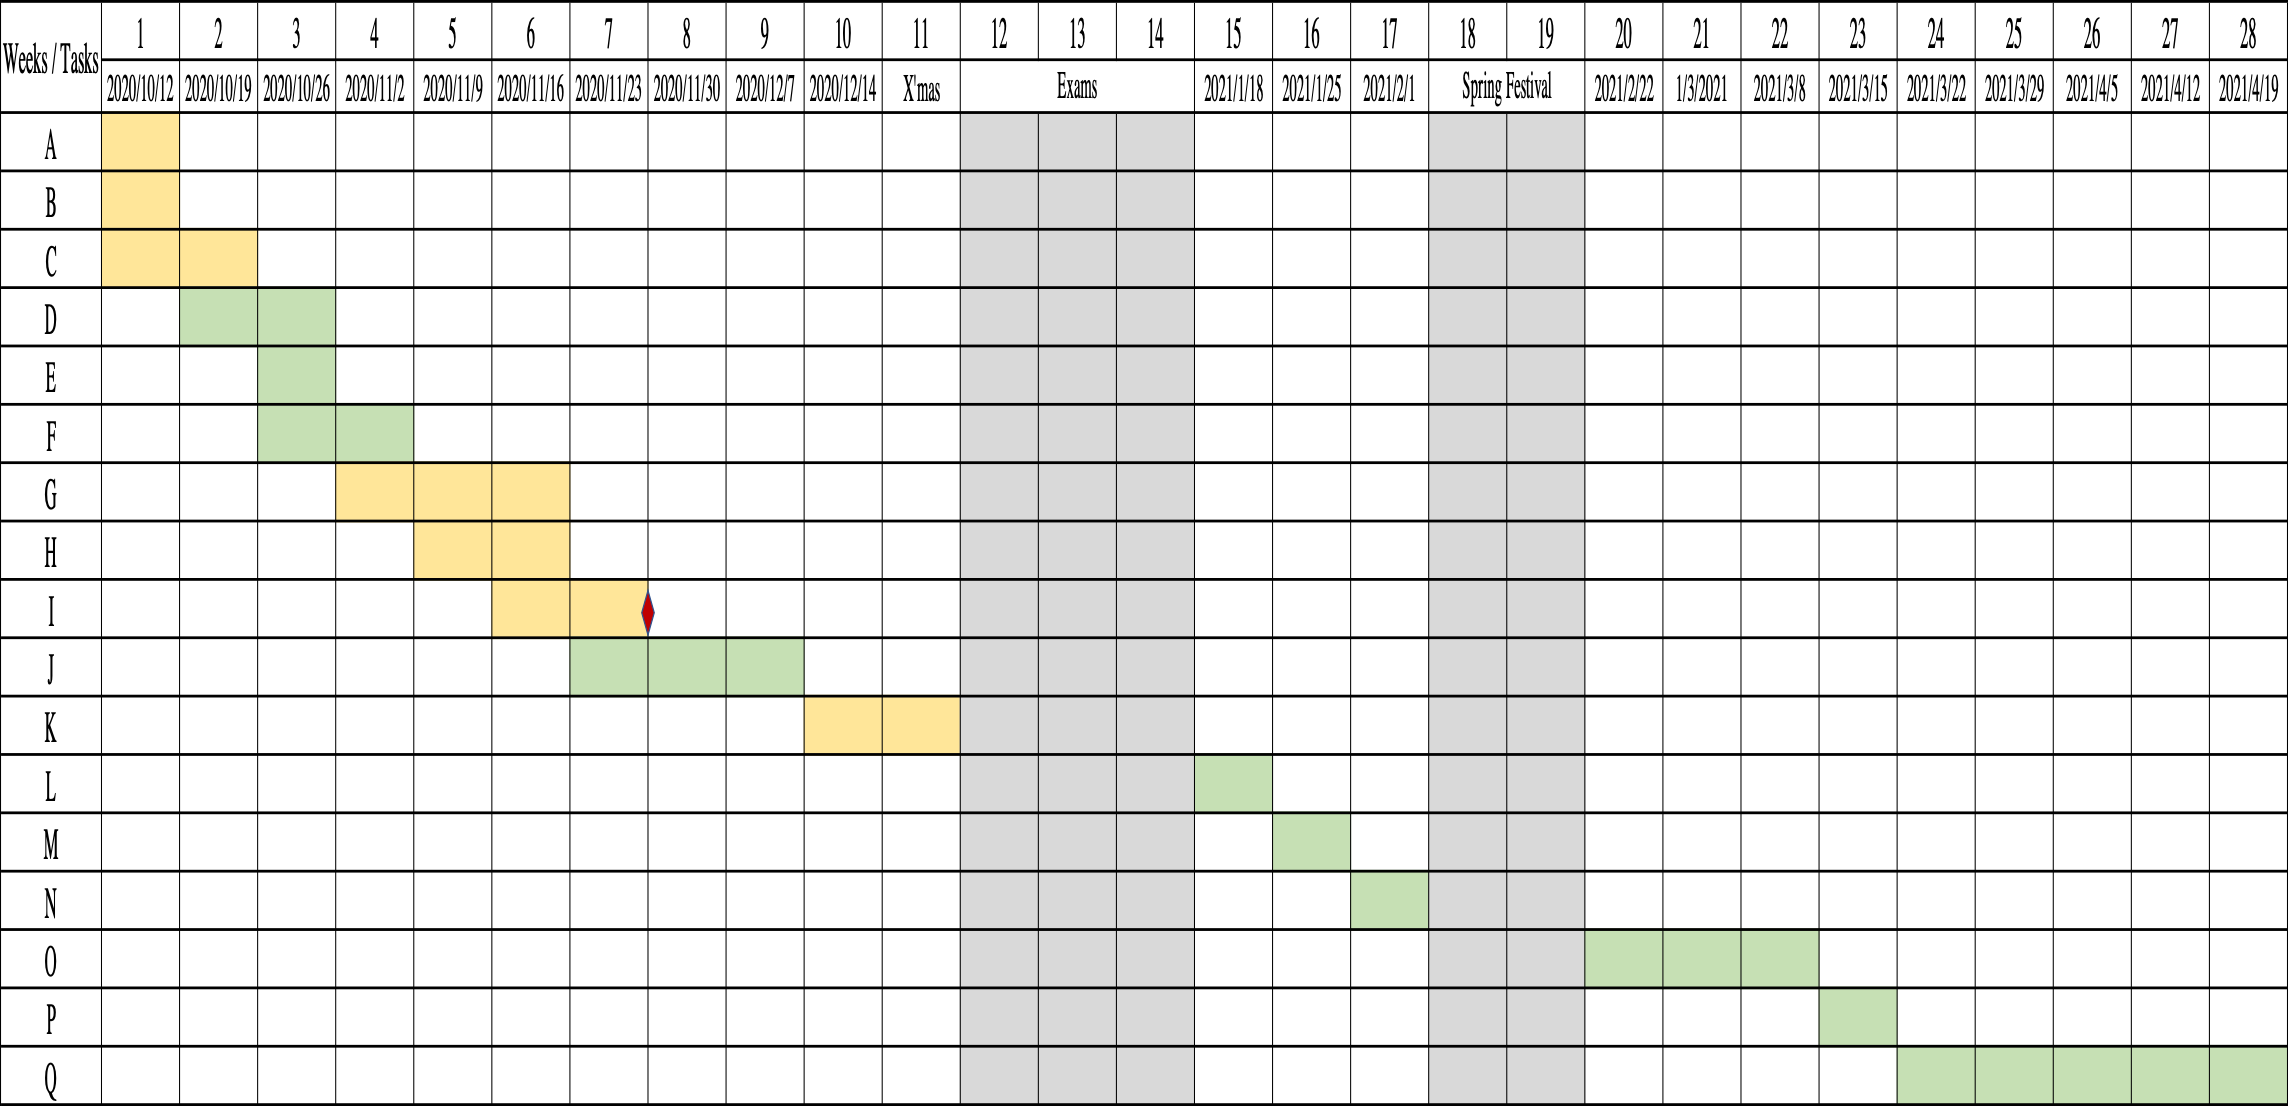
\includegraphics[width=1\textwidth]{images/original_plan.png}
    \caption{Original  Work Plan}
    \label{fig:10}
\end{figure}

\begin{figure}[H]
\centering
\subfigure[Timeline of Autumn Semester]{
    \begin{minipage}[b]{1.0\textwidth}
        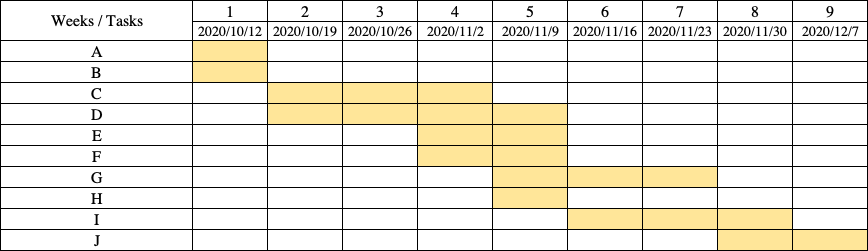
\includegraphics[width=1\textwidth]{images/timeline_autumn.png}
    \end{minipage}
}
\subfigure[Timeline of Spring Semester]{
    \begin{minipage}[b]{1.0\textwidth}
        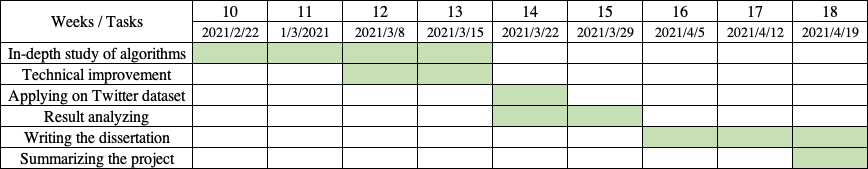
\includegraphics[width=1\textwidth]{images/timeline_spring.png}
    \end{minipage}
}

\caption{Actual Timeline}
\label{fig:11}
\end{figure}

Comparing with the original work-plan, the actual project progress is generally similar to it. The meetings with the supervisor were held every two weeks, which means that nearly every two weeks, the project moved to the next stage as schedule. The project progresses can be divided into two parts. The work of the first half of the project was mainly about basic research and data preparation. Though there were some unexpected reasons such as the limitations of Twitter API, data collecting and preprocessing parts have been still finished in the Autumn semester. As for the Spring semester, the work turned to study about the principles of the topic models and propose the technical improvement, because after communicated with the supervisor, we agreed that the implementation of the algorithm improvement is the basis of the following analysis of result and implementing a more suitable algorithm can make the result better. Therefore, we modified the original work plan to focus on the algorithm instead of directly applying the existing models on our Twitter dataset and analyzing the generated topics, also adjusted the order of the tasks. Figure \ref{fig:11} shows the actual project timeline, where the first one is for the Autumn semester and the second one is for the Spring semester (except exam weeks, Christmas and the Spring festival). 


\section{Achievements \& Contributions}\label{achievement}
In this project, we proposed a framework for uncovering COVID-19 events by analyzing social media data. The main contribution of this project can be divided into two parts, technical improvements on traditional topic models and applying the topic model on COVID-19 related dataset. 

Firstly, we proposed methods to collect COVID-19 related data from Twitter for creating our own dataset, and implement a framework to preprocess the data. Then, based on the research and experiments about text clustering algorithms, we had an in-depth study about the principles and derivations of different models and compared the efficiency of them. With a depth understanding of the algorithms, we proposed our own model based on the traditional topic model to implement the topic extraction of COVID-19 related Tweets. Though there still are some limitations, such as the impact of high-frequency words, the experimental results showed the performance of our model is better than traditional BTM on the test dataset and some more latent topics can be discovered. Moreover, under this framework, we can discover the events during different periods of the COVID-19 pandemic through extracting the latent topics, which is a new application area for topic models. And the analysis results for the evolution of the topics in different periods can be applied in other research areas such as sociology and anthropology. 

\section{Reflection \& Future Work}

Overall, the actual project progress generally accords with the work plan and all deadlines were submitted on time. Throughout the first half part of the project, there indeed were some outcomes. The codes for data collection and data preprocessing were finished and the data set were preliminarily built up. But because of the clear objectives of the project, we started the data preparing part and ignored intensively reading related papers, which made the subsequent work for algorithm implementation progressed slowly, and made it harder to understand and improve the topic models in the Spring semester. Fortunately, we did not encounter any unexpected problems during the process of developing in the Spring semester. We reserved enough time to write the dissertation and summarize the whole project. Consequently, though the project is completed on time, it can be more reasonable for the task management of some parts, for example, it should take more time to read the related papers before coding, which can make the following development more smoothly.

In the future, as mentioned in section \ref{application}, the first problem we need to focus on is to find more diverse datasets for training to improve the inference ability of our model and apply to a Twitter dataset covered the longer period of time during the pandemic. Subsequently, as mentioned in section \ref{achievement}, analyzing the generated topics in different periods of the pandemic can be used in sociology and anthropology research and the social media analysis can help government understand the public opinion to take the timely emergency response and take appropriate management measures during the pandemic \cite{han2020using}. Lee et al. \cite{lee2013real} proposed a real-time disease surveillance system, which combines geographical analysis, temporal analysis and text analysis together to automatically track disease activities and has real-time visualized output. It can be considered as the future direction of our project. With the current achievement on text analysis, in the next stage, we hope to propose a dynamic model and achieve a more advanced surveillance system for epidemic disease. 
